\documentclass{standalone}
\usepackage{tikz}
\usetikzlibrary{patterns, positioning}
\usepackage[sfdefault]{ClearSans} %% option 'sfdefault' activates Clear Sans as the default text font
\usepackage[T1]{fontenc}

\begin{document}
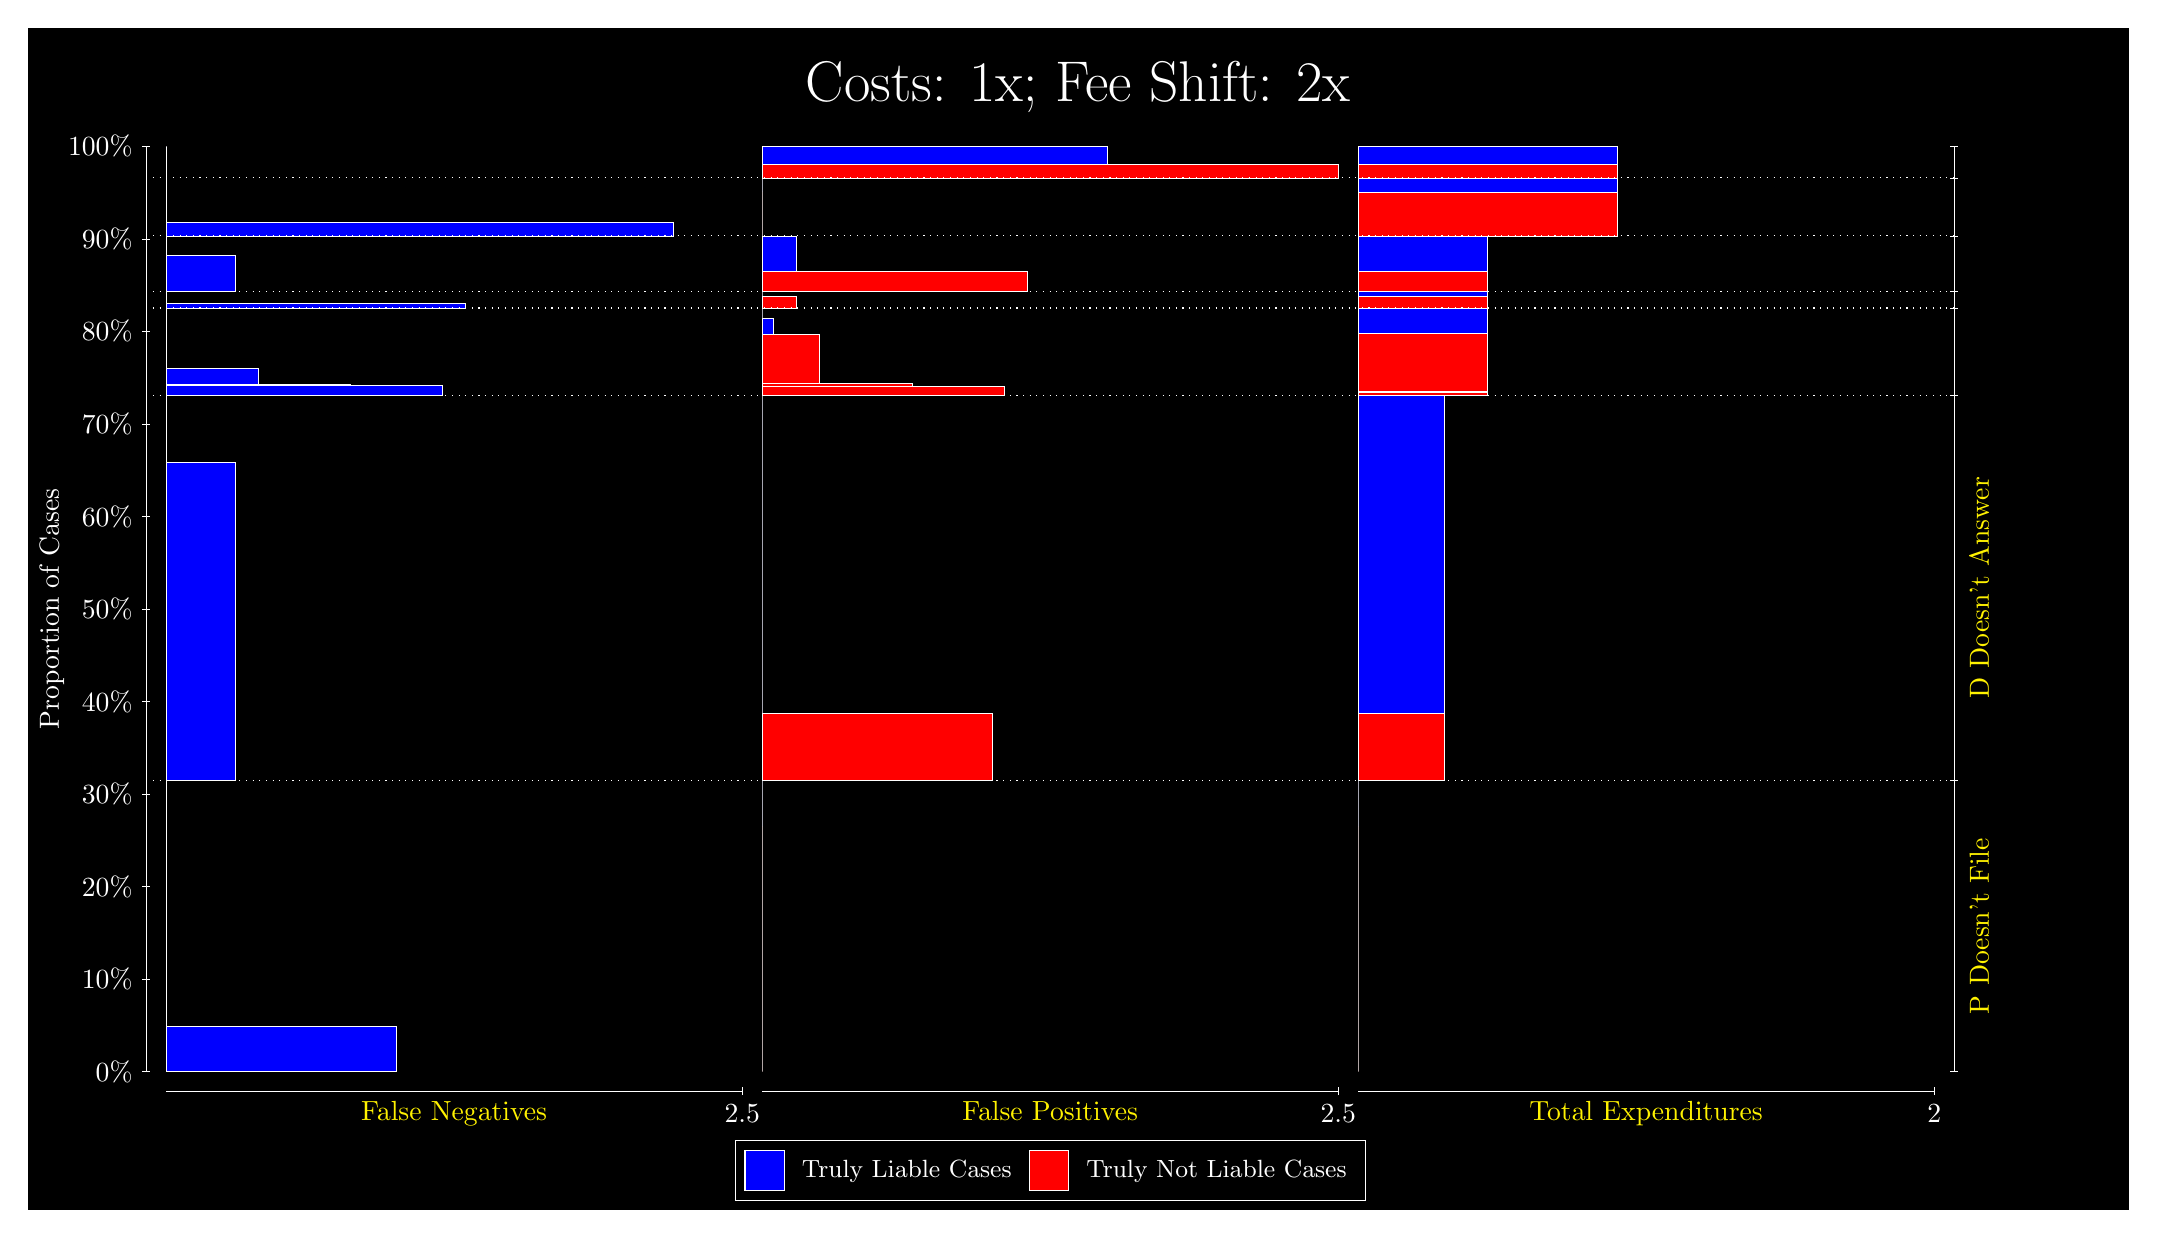
\begin{tikzpicture}
\draw[fill=black] (0,0) rectangle (26.667,15);
\draw[text=white] (0,13.5) rectangle (26.667,15) node[midway] {\huge Costs: 1x; Fee Shift: 2x};
\draw[white, very thin] (1.5,1.75) -- (1.5,13.5);
\node[rotate=90, text=white, anchor=center] at (0.3, 7.625) {Proportion of Cases};
\draw[white, very thin] (1.45,1.75) -- (1.55,1.75);
\node[text=white, anchor=east] at (1.45, 1.75) {0\%};
\draw[white, very thin] (1.45,2.925) -- (1.55,2.925);
\node[text=white, anchor=east] at (1.45, 2.925) {10\%};
\draw[white, very thin] (1.45,4.1) -- (1.55,4.1);
\node[text=white, anchor=east] at (1.45, 4.1) {20\%};
\draw[white, very thin] (1.45,5.275) -- (1.55,5.275);
\node[text=white, anchor=east] at (1.45, 5.275) {30\%};
\draw[white, very thin] (1.45,6.45) -- (1.55,6.45);
\node[text=white, anchor=east] at (1.45, 6.45) {40\%};
\draw[white, very thin] (1.45,7.625) -- (1.55,7.625);
\node[text=white, anchor=east] at (1.45, 7.625) {50\%};
\draw[white, very thin] (1.45,8.8) -- (1.55,8.8);
\node[text=white, anchor=east] at (1.45, 8.8) {60\%};
\draw[white, very thin] (1.45,9.975) -- (1.55,9.975);
\node[text=white, anchor=east] at (1.45, 9.975) {70\%};
\draw[white, very thin] (1.45,11.15) -- (1.55,11.15);
\node[text=white, anchor=east] at (1.45, 11.15) {80\%};
\draw[white, very thin] (1.45,12.325) -- (1.55,12.325);
\node[text=white, anchor=east] at (1.45, 12.325) {90\%};
\draw[white, very thin] (1.45,13.5) -- (1.55,13.5);
\node[text=white, anchor=east] at (1.45, 13.5) {100\%};

\draw[white, very thin] (24.457,1.75) -- (24.457,13.5);
\draw[white, very thin] (24.407,1.75) -- (24.507,1.75);
\node[anchor=west] at (24.407, 1.75) {};
\draw[white, very thin] (24.407,5.4435) -- (24.507,5.4435);
\node[anchor=west] at (24.407, 5.4435) {};
\draw[white, very thin] (24.407,10.339) -- (24.507,10.339);
\node[anchor=west] at (24.407, 10.339) {};
\draw[white, very thin] (24.407,11.447) -- (24.507,11.447);
\node[anchor=west] at (24.407, 11.447) {};
\draw[white, very thin] (24.407,11.657) -- (24.507,11.657);
\node[anchor=west] at (24.407, 11.657) {};
\draw[white, very thin] (24.407,12.362) -- (24.507,12.362);
\node[anchor=west] at (24.407, 12.362) {};
\draw[white, very thin] (24.407,13.1) -- (24.507,13.1);
\node[anchor=west] at (24.407, 13.1) {};
\draw[white, very thin] (24.407,13.5) -- (24.507,13.5);
\node[anchor=west] at (24.407, 13.5) {};

\draw[white, very thin, fill=blue] (1.75,1.75) rectangle (4.6775,2.3278);
\draw[white, very thin, fill=red] (1.75,2.3278) rectangle (1.75,5.4435);
\draw[white, very thin, fill=blue] (1.75,5.4435) rectangle (2.6283,9.484);
\draw[white, very thin, fill=red] (1.75,9.484) rectangle (1.75,10.339);
\draw[white, very thin, fill=blue] (1.75,10.339) rectangle (5.2631,10.459);
\draw[white, very thin, fill=blue] (1.75,10.459) rectangle (4.092,10.474);
\draw[white, very thin, fill=blue] (1.75,10.474) rectangle (2.921,10.677);
\draw[white, very thin, fill=red] (1.75,10.677) rectangle (1.75,11.447);
\draw[white, very thin, fill=blue] (1.75,11.447) rectangle (5.5558,11.509);
\draw[white, very thin, fill=red] (1.75,11.509) rectangle (1.75,11.657);
\draw[white, very thin, fill=blue] (1.75,11.657) rectangle (2.6283,12.112);
\draw[white, very thin, fill=red] (1.75,12.112) rectangle (1.75,12.362);
\draw[white, very thin, fill=blue] (1.75,12.362) rectangle (8.1906,12.541);
\draw[white, very thin, fill=red] (1.75,12.541) rectangle (1.75,13.1);
\draw[white, very thin, fill=red] (1.75,13.1) rectangle (1.75,13.277);
\draw[white, very thin, fill=blue] (1.75,13.277) rectangle (1.75,13.5);
\draw[white, very thin, fill=red] (9.3189,1.75) rectangle (9.3189,4.8657);
\draw[white, very thin, fill=blue] (9.3189,4.8657) rectangle (9.3189,5.4435);
\draw[white, very thin, fill=red] (9.3189,5.4435) rectangle (12.246,6.2989);
\draw[white, very thin, fill=blue] (9.3189,6.2989) rectangle (9.3189,10.339);
\draw[white, very thin, fill=red] (9.3189,10.339) rectangle (12.393,10.454);
\draw[white, very thin, fill=red] (9.3189,10.454) rectangle (11.222,10.486);
\draw[white, very thin, fill=red] (9.3189,10.486) rectangle (10.051,11.109);
\draw[white, very thin, fill=blue] (9.3189,11.109) rectangle (9.4652,11.313);
\draw[white, very thin, fill=blue] (9.3189,11.313) rectangle (9.3189,11.447);
\draw[white, very thin, fill=red] (9.3189,11.447) rectangle (9.758,11.595);
\draw[white, very thin, fill=blue] (9.3189,11.595) rectangle (9.3189,11.657);
\draw[white, very thin, fill=red] (9.3189,11.657) rectangle (12.686,11.907);
\draw[white, very thin, fill=blue] (9.3189,11.907) rectangle (9.758,12.362);
\draw[white, very thin, fill=red] (9.3189,12.362) rectangle (9.3189,12.921);
\draw[white, very thin, fill=blue] (9.3189,12.921) rectangle (9.3189,13.1);
\draw[white, very thin, fill=red] (9.3189,13.1) rectangle (16.638,13.277);
\draw[white, very thin, fill=blue] (9.3189,13.277) rectangle (13.71,13.5);
\draw[white, very thin, fill=red] (16.888,1.75) rectangle (16.888,4.8657);
\draw[white, very thin, fill=blue] (16.888,4.8657) rectangle (16.888,5.4435);
\draw[white, very thin, fill=red] (16.888,5.4435) rectangle (17.986,6.2989);
\draw[white, very thin, fill=blue] (16.888,6.2989) rectangle (17.986,10.339);
\draw[white, very thin, fill=red] (16.888,10.339) rectangle (18.534,10.371);
\draw[white, very thin, fill=blue] (16.888,10.371) rectangle (18.534,10.385);
\draw[white, very thin, fill=red] (16.888,10.385) rectangle (18.534,11.123);
\draw[white, very thin, fill=blue] (16.888,11.123) rectangle (18.534,11.447);
\draw[white, very thin, fill=red] (16.888,11.447) rectangle (18.534,11.595);
\draw[white, very thin, fill=blue] (16.888,11.595) rectangle (18.534,11.657);
\draw[white, very thin, fill=red] (16.888,11.657) rectangle (18.534,11.907);
\draw[white, very thin, fill=blue] (16.888,11.907) rectangle (18.534,12.362);
\draw[white, very thin, fill=red] (16.888,12.362) rectangle (20.181,12.921);
\draw[white, very thin, fill=blue] (16.888,12.921) rectangle (20.181,13.1);
\draw[white, very thin, fill=red] (16.888,13.1) rectangle (20.181,13.277);
\draw[white, very thin, fill=blue] (16.888,13.277) rectangle (20.181,13.5);
\draw[white, dotted] (1.5,5.4435) -- (24.457,5.4435);
\draw[white, dotted] (1.5,10.339) -- (24.457,10.339);
\draw[white, dotted] (1.5,11.447) -- (24.457,11.447);
\draw[white, dotted] (1.5,11.657) -- (24.457,11.657);
\draw[white, dotted] (1.5,12.362) -- (24.457,12.362);
\draw[white, dotted] (1.5,13.1) -- (24.457,13.1);
\draw[white, very thin] (1.75,1.5) -- (9.0689,1.5);
\node[text=yellow, anchor=north] at (5.4094, 1.5) {False Negatives};
\draw[white, very thin] (9.0689,1.45) -- (9.0689,1.55);
\node[text=white, anchor=north] at (9.0689, 1.45) {2.5};

\draw[white, very thin] (9.3189,1.5) -- (16.638,1.5);
\node[text=yellow, anchor=north] at (12.978, 1.5) {False Positives};
\draw[white, very thin] (16.638,1.45) -- (16.638,1.55);
\node[text=white, anchor=north] at (16.638, 1.45) {2.5};

\draw[white, very thin] (16.888,1.5) -- (24.207,1.5);
\node[text=yellow, anchor=north] at (20.547, 1.5) {Total Expenditures};
\draw[white, very thin] (24.207,1.45) -- (24.207,1.55);
\node[text=white, anchor=north] at (24.207, 1.45) {2};

\node[text=yellow, centered, rotate=90] at (24.777, 3.5968) {P Doesn't File};
\node[text=yellow, centered, rotate=90] at (24.777, 7.8915) {D Doesn't Answer};






\draw (12.978300999999998,1.5) node[draw=none] (baseCoordinate) {};
\begin{scope}[align=center]
        \matrix[scale=0.5, draw=white, below=0.5cm of baseCoordinate, nodes={draw}, column sep=0.1cm]{
            \node[rectangle, draw, minimum width=0.5cm, minimum height=0.5cm, fill=blue] {}; &
            \node[draw=none, font=\small, text=white] (B) {Truly Liable Cases}; &
            \node[rectangle, draw, minimum width=0.5cm, minimum height=0.5cm, fill=red] {}; &
            \node[draw=none, font=\small, text=white] (B) {Truly Not Liable Cases}; \\
            };
\end{scope}

\end{tikzpicture}
\end{document}